%Template file for a presentation using Latex and beamer
%You will need to install Latex, the beamer package, and some of these other packages on your own.
\documentclass[11pt,compress]{beamer} %slides and notes
\usepackage{amsmath,datetime,array,alltt,graphicx,xmpmulti,mathtools,bbm,booktabs,xspace,mathabx,tikz,pifont,epstopdf,relsize,wedn,hyperref,framed}
\usepackage[justification=centering]{caption}
\usepackage{subcaption}\captionsetup{compatibility=false}
\usepackage[autolinebreaks]{mcodefred}
\usepackage[author-year]{amsrefs}
\usepackage{qtree}
\usepackage{pst-node}% http://ctan.org/pkg/pst-node
\usepackage{textcomp} %helps to compile MATLAB code in mcode or lstlisting
\usepackage{pgf,pgfarrows,pgfnodes} % Drawing tables, arrows, ...
\usepackage[customcolors]{hf-tikz} % Box equations
\input FJHDef.tex


\newcommand{\HickernellFJ}{Hickernell} %To give my name to the bibliography

\newtheorem{lem}{Lemma}
\setbeamertemplate{theorems}[numbered]

\usetikzlibrary{arrows}
\newcommand*\circled[1]{\tikz[baseline=(char.base)]{
  \node[shape=circle,color=green,draw,inner sep=1pt] (char) {#1};}}
\setlength{\parskip}{2ex}
\setlength{\arraycolsep}{0.5ex}
\newcommand{\tol}{\text{tol}}
\newcommand{\e}{\text{e}}
\DeclareMathOperator{\cubMC}{cubMC}
\DeclareMathOperator{\qse}{qse}
\DeclareMathOperator{\integ}{int}
\DeclareMathOperator{\trap}{trap}
\DeclareMathOperator{\size}{size}
\DeclareMathOperator{\app}{id}
\DeclareMathOperator{\err}{err}
\DeclareMathOperator{\walsh}{walsh}
\newcommand{\happ}{\widehat{\app}}
\newcommand{\hinteg}{\widehat{\integ}}
\newcommand{\cube}{[0,1)^d}
\newcommand{\desall}{\{\vx_i\}}
\newcommand{\desn}{\{\vz_i\}_{i=0}^{n-1}}
\def\newblock{\hskip .11em plus .33em minus .07em}
\newcommand{\wcS}{\widecheck{S}}
\newcommand{\wcomega}{\widecheck{\omega}}
\newcommand{\prob}[1]{\mathbb{P}\left( #1 \right)}
\newcommand{\bsk}{\boldsymbol{k}}    % vector k
\newcommand{\bsz}{\boldsymbol{z}}    % vector z
\newcommand{\bsx}{\boldsymbol{x}}    % vector z
\newcommand{\F}{\mathbb{F}} % field, finite field
\newcommand{\bsDelta}{\boldsymbol{\Delta}}    % vector
\newcommand{\bszero}{\boldsymbol{0}} % vector of zeros
\newcommand{\E}{{\rm e}}
\newcommand{\D}{{\rm d}}
\newcommand{\Z}{\mathbb{Z}}
\newcommand{\R}{\mathbb{R}}
\newcommand{\N}{\mathbb{N}}
\newcommand{\I}{\mathsf{I}}
\DeclareMathOperator{\Var}{Var}
\DeclareMathOperator{\affine}{affine}
\DeclareMathOperator{\Genz}{Genz}
\DeclareMathOperator{\payoff}{payoff}
\newcommand{\intalg}{\widehat{\mu}\left(\vx\mapsto f(\vx),\varepsilon\right)}

\newcommand*{\Scale}[2][4]{\scalebox{#1}{$#2$}}%
\newcommand{\sqdiamond}[1][fill=gray_plot]{\tikz [x=1.2ex,y=1.85ex,line width=.1ex,line join=round, yshift=-0.285ex] \draw  [#1]  (0,.5) -- (.5,1) -- (1,.5) -- (.5,0) -- (0,.5) -- cycle;}%

\definecolor{orange_plot}{rgb}{1.,.5,.0}
\definecolor{gray_plot}{rgb}{.7,.7,.7}
\definecolor{green_plot}{rgb}{.0,.5,.0}


\usetheme{FredIIT}
% \usetheme{Berlin}
\logo{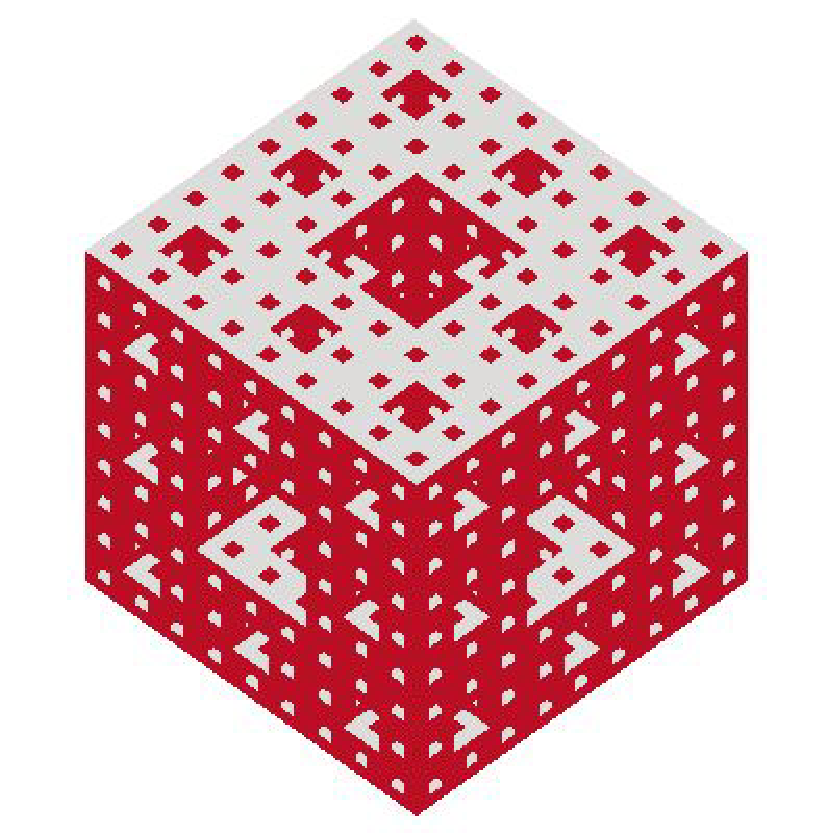
\includegraphics[width=1cm]{MengerIITRedGray.pdf}}

\title[MCM 2017]{Automatic estimation of first-order Sobol' indices using the replication procedure}
\author[ljimene1@hawk.iit.edu]{Llu\'is Antoni Jim\'enez Rugama, Laurent Gilquin,\\ \'Elise Arnaud, Fred J. Hickernell,\\ Herv\'e Monod, Cl\'ementine Prieur}
\institute{
%Room 208, Bldg E1, Department of Applied Mathematics \\
%Illinois Institute of Technology, Chicago, 60616 IL \\
Illinois Institute of Technology\\
Email: \href{mailto:ljimene1@hawk.iit.edu}{\url{ljimene1@hawk.iit.edu}}}
%Website: \url{http://math.iit.edu/~lantoni/}
% \date[{Revised \currenttime, \mdyyyydate \today}]{Revised \settimeformat{ampmtime} \currenttime, \today}
\date[]{Wednesday ${\rm{5^{th}}}$ July, 2017}
%{Monday ${\rm{28^{th}}}$ September, 2015}

\begin{document}
\frame{\titlepage}

%\frame{\frametitle{Outline}\begin{minipage}{15cm}\tableofcontents\end{minipage}}
%\AtBeginSection[]
%{ \begin{frame}
%  \frametitle{Outline}
%  \begin{minipage}{15cm}
%  \tableofcontents[currentsection]
%  \end{minipage}
%  \end{frame}
%}

\begin{frame}<0>[label = Outline]\frametitle{Outline}
\begin{itemize}
\item<1,2> \alert<2>{Sobol' Indices}\only<2>{---What are they?}
%\item<1,2-3> \alert<2,3>{Introduction}
%\begin{itemize}
%\item<1,2> \alert<2>{ANOVA}\only<2>{---The ANalysis Of VAriance decomposition.}
%\item<1,3> \alert<3>{Sobol' Indices}\only<3>{---Measuring the importance of each input.}
%\end{itemize}
\item<1,3> \alert<3>{Quasi-Monte Carlo Methods}\only<3>{---How can we estimate 
$S_u$ efficiently?}
\item<1,4> \alert<4>{Replication Procedure}\only<4>{---Reducing the number of function evaluations to compute \emph{first-order} indices.}
\end{itemize}
\end{frame}

\section{Sobol Indices'}
\setbeamercovered{transparent = 50} % Translucid <only>
\againframe<2>{Outline}
\setbeamercovered{invisible} % Invisible <only>


\begin{frame}
\frametitle{ANOVA}
For $f\in L^2\left([0,1]^d\right)$, and $1\!:\!d=\{1,\dots,d\}$,
\begin{equation*}
f(\vx)=\sum \limits_{u \subseteq 1:d} f_u(\vx)\, , \qquad f_{\varnothing} = \mu\, ,
\label{anova}
\end{equation*}
where,
\[f_u(\vx)= \int_{[0,1]^{d-|u|}} f(\vx) d{\vx}_{-u} - \sum \limits_{v \subset u} f_v(\vx)\, .\]

\vspace{-2ex}
\begin{itemize}
\item $\abs{u}$ the cardinality of $u$.
\item $-u:=u^c=1\!:\!d \, \setminus \, u$.
\end{itemize}

\vspace{-5ex}

\begin{multline*}
\text{e.g.\ } \underbrace{\E^{x_1} \cos(x_2)}_{f(x)} 
= \underbrace{(\E - 1)\sin(1)}_{f_\emptyset} 
+ \underbrace{(\E^{x_1} - \E + 1)\sin(1)}_{f_{\{1\}}} \\
+ \underbrace{(\E - 1)(\cos(x) - \sin(1))}_{f_{\{2\}}} 
+ \underbrace{(\E^{x_1} - \E + 1)(\cos(x) - \sin(1))}_{f_{\{1,2\}}}
\end{multline*}
\end{frame}

\begin{frame}
\frametitle{Variance decomposition}
Under the previous definitions,
\begin{equation*}
\sigma^2_{\varnothing} = 0\, ,\qquad \sigma^2_{u} =\int_{[0,1]^{d}} f_u(\vx)^2 d{\vx}\, ,\qquad \sigma^2 =\int_{[0,1]^{d}} \left(f(\vx)-\mu\right)^2 d{\vx}\, .
\end{equation*}
The ANOVA identity is,

\[
\sigma^2 = \sum \limits_{u \subseteq 1:d} \sigma_u^2 \, .
\]
\end{frame}

\begin{frame}
\frametitle{Sobol' indices}
Sobol' 
\ycite{Sob90} and \ycite{Sob01} 
introduced the \emph{global sensitivity} indices which 
measure the variance 
explained by any dimension subset $u \subseteq 1\!:\!d$:
\begin{equation*}
\underline{\tau}_u^2 = \sum_{\substack{v \subseteq u \\ v\,\subseteq 1:d}} \sigma_v^2\, , 
\quad \text{ and } \quad \overline{\tau}_u^2 = \sum_{\substack{v \cap u\neq\varnothing \\ 
v\,\subseteq 1:d}} \sigma_v^2\, .
\end{equation*}
We have the following properties,
\begin{itemize}
\item $\underline{\tau}_u^2\leq \overline{\tau}_u^2$.
\item $\underline{\tau}_u^2 + \overline{\tau}_{-u}^2 =\sigma^2$.
\end{itemize}
\end{frame}

\begin{frame}
\frametitle{Normalized closed first-order Sobol' indices}
From now on, we consider the normalized Sobol' indices and $|u|=1$,
\setbeamercovered{transparent} % Translucid <only>
\begin{gather*}
S_{u}=\frac{\underline{\tau}_u^{2}}{\sigma^2}=1-\frac{\displaystyle 
\int_{[0,1]^{2d-1}}f(\vx)\bigl(f(\vx)-f(\vx_u:{\vx'}_{-u})\bigr)
 d\vx d{\vx'}_{-u}}{\displaystyle \int_{[0,1]^d} f(\vx)^2 d{\vx}-\left(\int_{[0,1]^d} f(\vx) 
 d{\vx}\right)^2},
\end{gather*}
satisfying $
0\leq S_{u} \leq 1$. More specifically, $S_{u}$ is composed by,
\vspace{-0.2cm}
\begin{equation*}
S_{u}=1-\frac{\mu_1}{\mu_2-\mu_3^2},\quad \text{where }\begin{cases}\mu_1\text{ is a 
}2d-1\text{ dim. integral.} \\ \mu_2\text{ is a }d\text{ dim. integral.} \\ \mu_3\text{ is a 
}d\text{ dim. integral.} \end{cases}
\end{equation*}
\vspace{-0.3cm}
Error bounds for $S_{u}$ require more care than error bounds for the $\mu_j$.
\end{frame}

\begin{frame}
\frametitle{Improving the estimator}
Suppose that $\boldsymbol{\mu}:=(\mu_1, \mu_2, \mu_3) \in  
[\widehat{\boldsymbol{\mu}}-\textbf{err}, \widehat{\boldsymbol{\mu}}+\textbf{err}]$ for 
\[
\hmu_j = \frac 1n \sum_{i=0}^{n-1} g_j(\boldsymbol{x}_i)
\]
and some data-based $\widehat{\boldsymbol{\mu}}$ and $\textbf{err}$. A 
natural way to estimate $S_{u}$ is 
\begin{equation*}
\widehat{S}_{u} = 1 - \frac{\widehat{\mu}_1}{\widehat{\mu}_2-\widehat{\mu}_3^2},
\end{equation*}
Nonetheless, 
\begin{equation*}
\widetilde{S}_{u}=1 - \frac{1}{2}\left(\max_{\boldsymbol{\mu} \in  
[\boldsymbol{\widehat{\mu}}-\textbf{err}, 
\boldsymbol{\widehat{\mu}}+\textbf{err}]}\frac{\mu_1}{\mu_2-\mu_3^2} + 
\min_{\boldsymbol{\mu} \in  [\boldsymbol{\widehat{\mu}}-\textbf{err}, 
\boldsymbol{\widehat{\mu}}+\textbf{err}]}\frac{\mu_1}{\mu_2-\mu_3^2} \right),
\end{equation*}
guarantees the tightest absolute error bound.
\end{frame}

\begin{frame}
\frametitle{Why?}
%Contrary to $\widehat{S}_{u}$, $\widetilde{S}_{u}$ guarantees the tightest error bound.
%\begin{equation*}
%|S_u - \widetilde{S}_{u}| \leq \frac{1}{2}\left(\max_{\boldsymbol{\mu} \in  [\boldsymbol{\widehat{\mu}}-\textbf{err}, \boldsymbol{\widehat{\mu}}+\textbf{err}]}\frac{\mu_1}{\mu_2-\left(\mu_3\right)^2} - \min_{\boldsymbol{\mu} \in  [\boldsymbol{\widehat{\mu}}-\textbf{err}, \boldsymbol{\widehat{\mu}}+\textbf{err}]}\frac{\mu_1}{\mu_2-\left(\mu_3\right)^2} \right).
%\end{equation*}

For instance, if $\boldsymbol{\mu}\in[1,1]\times[1,3]\times[0,0]$, then
\begin{align*}
\frac{1}{3} & \le S_u \le 1, \\
\bigl |S_u - \widehat{S}_{u} \bigr | & = \biggl |S_u - \frac 12 \biggr |\leq \frac 12 , \\
\bigl |S_u - \widetilde{S}_{u} \bigr | & = \biggl |S_u -\frac 23 \biggl |\leq \frac 13,
\end{align*}
In this case, $1/3$ is the smallest error bound possible.

A deeper study is provided in \cite{HicEtal17a} and \cite{GilJim16b}.
\end{frame}

\section{Quasi-Monte Carlo Methods}
\setbeamercovered{transparent} % Translucid <only>
\againframe<3>{Outline}
\setbeamercovered{invisible} % Invisible <only>

\begin{frame}
\frametitle{Adaptive quasi-Monte Carlo cubature}
To estimate $S_{u}$ using $\widetilde{S}_u$ we need to approximate $\mu_1$, 
$\mu_2$, 
and $\mu_3$ such that $\mu_j\in[\widehat{\mu}_j-\text{err}_j, 
\widehat{\mu}_j+\text{err}_j]$.

Assuming that integrands defining $\mu_1$, $\mu_2$, and $\mu_3$ satisfy some 
specific 
conditions on the decay of the Fourier coefficients, in \cite{HicJim16a} and 
\cite{JimHic16a} we provided two adaptive quasi-Monte Carlo cubatures that compute 
$\widehat{\mu}_{j,n}$ and $\text{err}_{j,n}$ such that
\begin{equation}\label{error_bound}
|\mu_j - \widehat{\mu}_{j,n}| \leq \text{err}_{j,n}
\end{equation}
Given the error tolerance $\varepsilon$, the number of points $n$ is increased until 
\[
\max_{\boldsymbol{\mu} 
	\in [\widehat{\boldsymbol{\mu}}_{j,n} - \textbf{err}_{j,n}, 
\widehat{\boldsymbol{\mu}}_{j,n} + \textbf{err}_{j,n}]} \
\bigl |S_u(\boldsymbol{\mu}) - \widetilde{S}_{u} \bigr | 
\le \varepsilon
\]
\end{frame}

\begin{frame}
\frametitle{Estimating $\mu_1$, $\mu_2$, and $\mu_3$ automatically}
Given $\varepsilon$ and $\vx\mapsto f(\vx)$, we want $\widehat{\mu}$ such that
\[
\abs{\int_{[0,1]^d} f(\bsx)\,\D\bsx - \intalg}\leq \varepsilon,
\]
where
\[
\intalg = \frac{1}{2^m} \sum_{i=0}^{2^m-1} f(\bsz_i\oplus\vDelta),
\]
for some \alert{automatic} choice of $m$ and $\{\bsz_i\}_{i=0}^{\infty}
\in\begin{Bmatrix}\textcolor{magenta}{\text{Lattice}}\\\textcolor{blue}{\text{Digital}}\end{Bmatrix}$ sequence.%, and
%\[
%\cost\left(\intalg\right)=\mathcal{O}\left((m+\$(f))2^m\right)
%\]
\end{frame}

\begin{frame}
\frametitle{Examples of sequences}
\begin{figure}\centering
\begin{subfigure}[b]{0.45\textwidth}
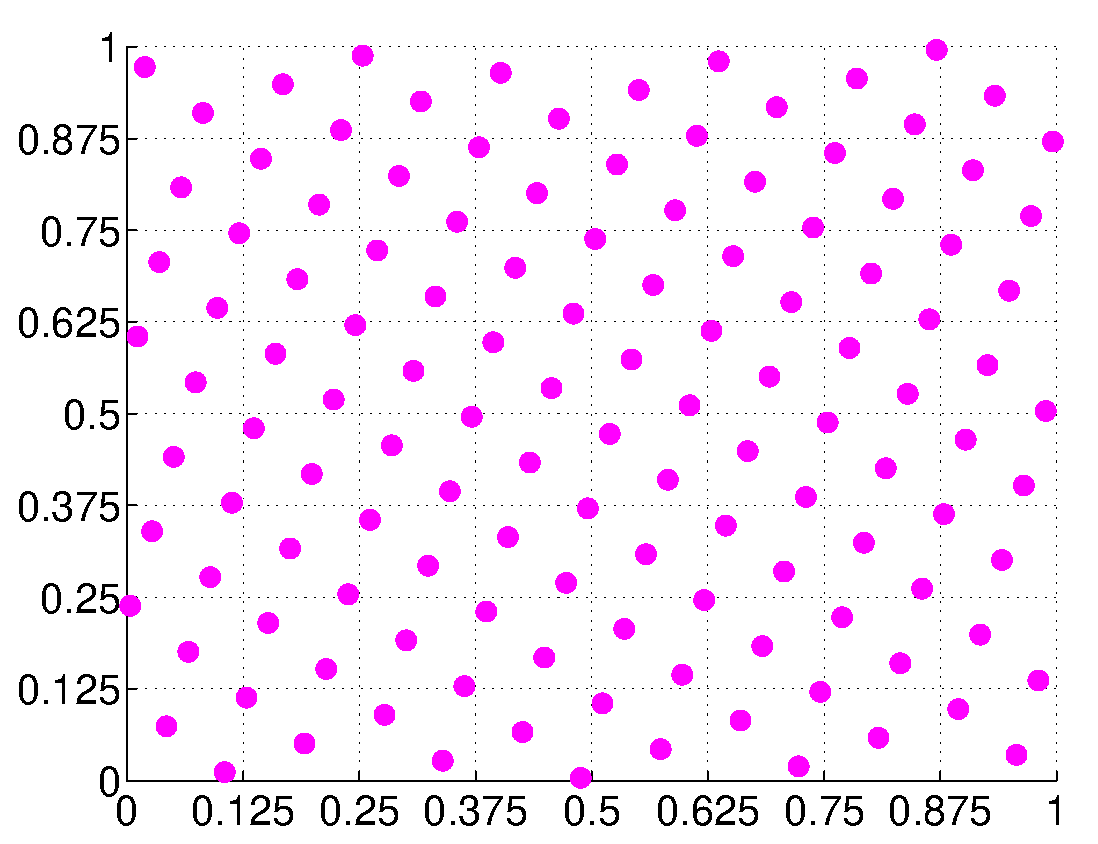
\includegraphics[width=1.\textwidth]{Images/lat_seq.eps}
\caption*{Shifted rank-1 lattice sequence with generating vector $(1,47)$.}
\end{subfigure}
~ % Spacing between figures
\begin{subfigure}[b]{0.45\textwidth}
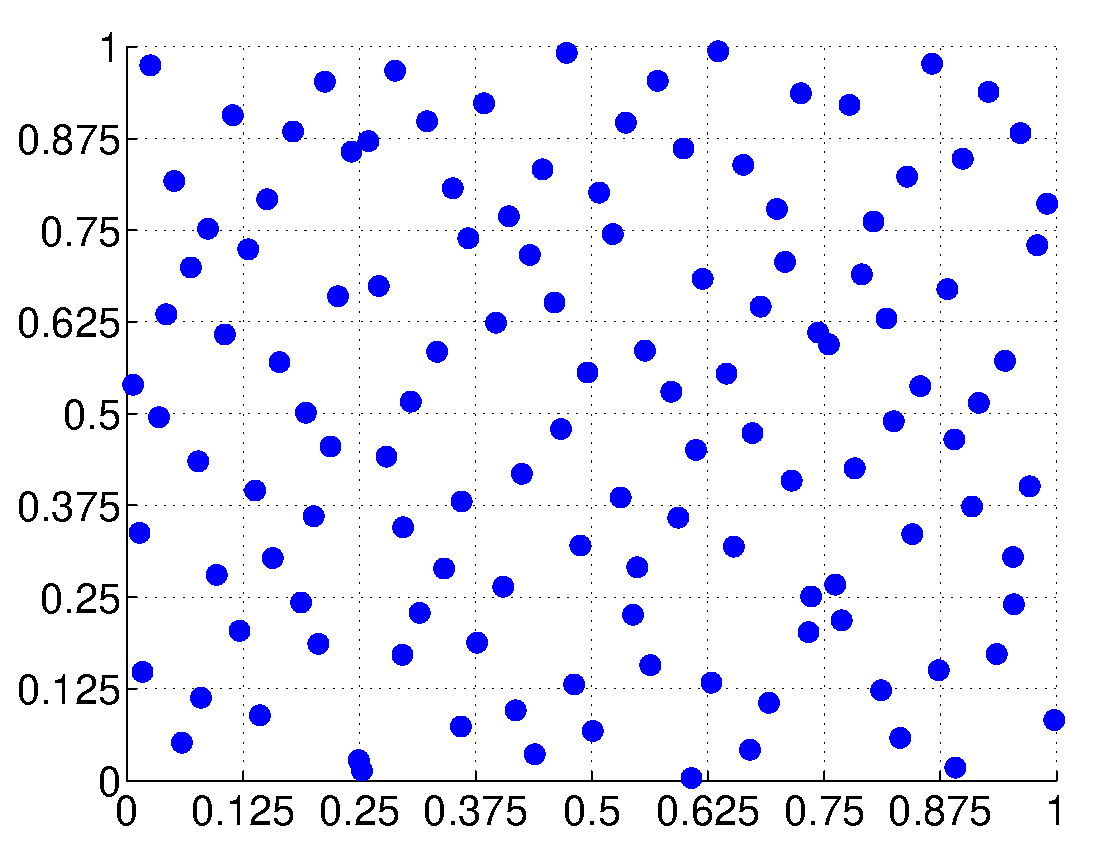
\includegraphics[width=1.\textwidth]{Images/sob_seq.eps}
\caption*{Digitally shifted scrambled Sobol' sequence.}
\end{subfigure}
\end{figure}
\end{frame}

\begin{frame}
\frametitle{Adaptive algorithm for integrands $f\in\cc$}
\[\Scale[0.90]{\displaystyle
\abs{\int_{[0,1]^d} f(\vx)\, d\vx - \frac{1}{2^m} \sum\limits_{i=0}^{2^m-1} f(\vx_i)} \leq 
\overbrace{\sum \textcolor{green_plot}{\boldsymbol{\newmoon}}}^{\substack{\text{Dual 
net/lat} \\ \text{Fourier coef}}} \leq \fC(r,m)\sum_{\kappa=\left \lfloor 2^{m-r-1}\right 
\rfloor}^{2^{m-r}-1} \bigabs{\tf_{m,\kappa}} \leq \varepsilon
}\]
\vspace{-.5cm}
\begin{columns}
\begin{column}{0.6\textwidth}
\centering
\begin{figure}
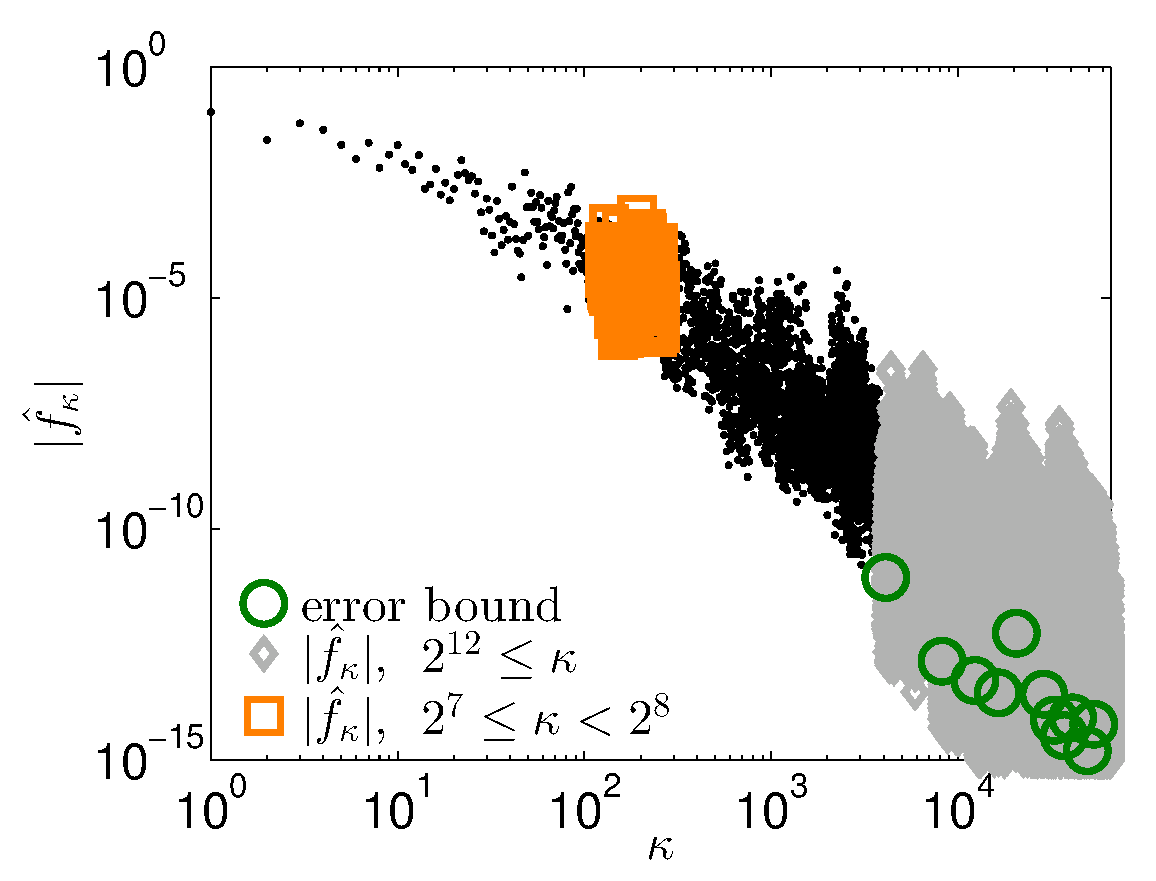
\includegraphics[width=.8\textwidth]{Images/WalshCoeffExplanation.eps}
\end{figure}
\end{column}
\begin{column}{0.4\textwidth}
\centering
$\cc=\begin{Bmatrix}\displaystyle\sum\textcolor{orange_plot}{\pmb{\blacksquare}}\text{ bounds }\sum\textcolor{gray_plot}{\boldsymbol{\sqdiamond}}\\
\displaystyle\sum\textcolor{gray_plot}{\boldsymbol{\sqdiamond}}\text{ bounds }\sum\textcolor{green_plot}{\boldsymbol{\newmoon}}\end{Bmatrix}$
\end{column}
\end{columns}
\end{frame}

\section{Replication Method}
\setbeamercovered{transparent} % Translucid <only>
\againframe<4>{Outline}
\setbeamercovered{invisible} % Invisible <only>

\begin{frame}
\frametitle{Number of function evaluations to estimate $\widetilde{S}_1,\dots,\widetilde{S}_d$}
Computing all the indices one by one, if one requires $n$ points for each estimation, the total number of function evaluations is
\[
2dn\, ,
\]
However, if all indices are computed together, some evaluations can be saved. Therefore, the number of function evaluations becomes
\[
(1+d)n\, ,
\]
Finally, under a special set of quasi-Monte Carlo sequences, this number can be decreased to
\[
2n\, .
\]
\end{frame}

\begin{frame}
\frametitle{Normalized first-order Sobol' indices}
Given $\vx,\vx'\in [0,1]^d$, we define the following point,
\begin{gather*}
(\vx_u:{\color{blue}\vx'_{-u}}) := 
({\color{blue}x'_1},\dots,{\color{blue}x'_{u-1}},x_u,{\color{blue}x'_{u+1}},\dots,{\color{blue}x'_d})\in
[0,1]^d.
\end{gather*}

This point is used in the definition of $S_u$:
\begin{equation*}
S_{u}=1-\frac{\displaystyle \int_{[0,1]^{2d-1}}f(\vx)\bigl (f(\vx) - 
	f(\vx_u:{\color{blue}{\vx'}_{-u}})\bigr) d\vx 
	d{\color{blue}{\vx'}_{-u}}}{\displaystyle\int_{[0,1]^d} f(\vx)^2 d{\vx}-\left(\int_{[0,1]^d} 
	f(\vx) 
	d{\vx}\right)^2}\, .
\end{equation*}
\end{frame}




\begin{frame}
\frametitle{Replicated designs}
For the cubature, we must evaluate 
\begin{gather*}
f(\vx_i)=f(x_{i,1},\dots,x_{i,u-1},x_{i,u},x_{i,u+1},\dots,x_{i,d})\, ,\\
f(\vx_{i,u},{\color{blue}\vx'_{i,-u}})=f({\color{blue}x'_{i,1}},\dots,{\color{blue}x'_{i,u-1}},
x_{i,u},{\color{blue}x'_{i,u+1}},\dots,{\color{blue}x'_{i,d}})\,
\end{gather*}
\alert{for all $u$}.  We show that $f(\vx_i)$ and $f({\color{blue}\vx'_{i}})$ are enough.  We 
focus on well 
uniformly distributed points $\vx_i$ and ${\color{blue}\vx'_i}$ such that,
\begin{equation*}
\begin{pmatrix}
x_{0,1} & \cdots & x_{0,d} \\
\vdots & \vdots & \vdots \\
x_{i,1} & \cdots & x_{i,d} \\
\vdots & \vdots & \vdots
\end{pmatrix},\qquad
\begin{pmatrix}
{\color{blue}x'_{0,1}} & \cdots & {\color{blue}x'_{0,d}} \\
\vdots & \vdots & \vdots \\
{\color{blue}x'_{i,1}} & \cdots & {\color{blue}x'_{i,d}} \\
\vdots & \vdots & \vdots
\end{pmatrix}=
\begin{pmatrix}
x_{{\color{blue}\pi_1(0)},1} & \cdots & x_{{\color{blue}\pi_d(0)},d} \\
\vdots & \ddots & \vdots \\
x_{{\color{blue}\pi_1(i)},1} & \cdots & x_{{\color{blue}\pi_d(i)},d} \\
\vdots &  & \vdots \\
\end{pmatrix}\, ,
\end{equation*}
where the permutations $\pi_u$  reorder the $\vx_{i,u}$ into the 
$\color{blue}\vx'_{i,u}$.
\end{frame}

\begin{frame}
\frametitle{Sobol' points}
By construction, Sobol' points have this property when $n=2^m$. For instance, if $d=2$ we can use a fourth dimensional Sobol' sequnce $\{\vz_i\}_{i\in\natzero}$:
\begin{equation*}
\begin{pmatrix}
z_1 & z_2 \\
x_1 & x_2 \\
0 & 0 \\
0.5 & 0.5  \\
0.25 & 0.75 \\
0.75 & 0.25 \\
0.125 & 0.625 \\
0.625 & 0.125 \\
0.375 & 0.375 \\
0.875 & 0.875 \\
\vdots & \vdots
\end{pmatrix},\qquad
\begin{pmatrix}
z_3 & z_4 \\
\color{blue} x'_1 & \color{blue} x'_2 \\
\color{blue} 0 & \color{blue} 0 \\
\color{blue} 0.5 & \color{blue} 0.5  \\
\color{blue} 0.25 & \color{blue} 0.75 \\
\color{blue} 0.75 & \color{blue} 0.25 \\
\color{blue} 0.875 & \color{blue} 0.875 \\
\color{blue} 0.375 & \color{blue} 0.375 \\
\color{blue} 0.625 & \color{blue} 0.125 \\
\color{blue} 0.125 & \color{blue} 0.625 \\
\vdots & \vdots
\end{pmatrix}, \qquad
\begin{pmatrix}
&& \\
\color{blue} \pi_1 & \color{blue} \pi_2 \\
\color{blue} 0 & \color{blue} 0 \\
\color{blue} 1 & \color{blue} 1 \\
\color{blue} 2 & \color{blue} 2 \\
\color{blue} 3 & \color{blue} 3 \\
\color{blue} 7 & \color{blue} 7 \\
\color{blue} 6 & \color{blue} 6 \\
\color{blue} 5 & \color{blue} 5 \\
\color{blue} 4 & \color{blue} 4 \\
\vdots & \vdots \\
\end{pmatrix}\, .
\end{equation*}
\end{frame}

\begin{frame}
\frametitle{No need to evaluate $f(\vx_{i,u}:{\color{blue}{\vx'}_{i,-u}})$ for $d$ 
different $u$}
Given the right order of our points $\color{blue}\vx'_i$ into $\vx_i$, i.e. $\color{blue}\pi^{-1}_u$:
\begin{equation*}
\begin{pmatrix}
{\color{blue}\vx'_{\pi^{-1}_u(0)}} \\
\vdots \\
{\color{blue}\vx'_{\pi^{-1}_u(n)}} \\
\vdots
\end{pmatrix}=
\begin{pmatrix}
{\color{blue}x'_{\pi^{-1}_u(0),1}} & \cdots & {x_{0,u}} & \cdots & {\color{blue}x'_{\pi^{-1}_u(0),d}} \\
\vdots & & \vdots & & \vdots \\
{\color{blue}x'_{\pi^{-1}_u(n),1}} & \cdots & x_{n,u} & \cdots & {\color{blue}x'_{\pi^{-1}_u(n),d}} \\
\vdots & & \vdots & & \vdots
\end{pmatrix}\, .
\end{equation*}
Thus, evaluating $f({\color{blue}\vx'_i})$, one can directly obtain the 
$f(\vx_{i,u}:{\color{blue}{\vx'}_{i,-u}})$:
\begin{equation*}
\begin{pmatrix}
f({\color{blue}\vx'_{0}}) \\
\vdots \\
f({\color{blue}\vx'_{i}}) \\
\vdots
\end{pmatrix}=
\begin{pmatrix}
\color{red} y_{0} \\
\vdots \\
\color{red} y_{i} \\
\vdots
\end{pmatrix} \Longrightarrow
\begin{pmatrix}
f(\vx_{0,u}:{\color{blue}{\vx'}_{0,-u}})\\
\vdots\\
f(\vx_{i,u}:{\color{blue}{\vx'}_{i,-u}})\\
\vdots\\
\end{pmatrix}:=
\begin{pmatrix}
\color{red} y_{\pi^{-1}_u(0)} \\
\vdots \\
\color{red} y_{\pi^{-1}_u(i)} \\
\vdots
\end{pmatrix}
\end{equation*}
\end{frame}

	\begin{frame}
\frametitle{Sobol' Indices Example from \ocite{BraFoxNie92}}
\vspace{-4ex}

\uncover<1>{
	\[
	f(\vx)=-x_1+x_1x_2-x_1x_2x_3+\dots + x_1 x_2x_3 x_4 x_5 x_6 
	\]
	\begin{gather*}
	\varepsilon = 1\text{E}{-3}, \qquad n =  65~536 \\
	\begin{array}{ r | ccccccc }
	%\varepsilon = 1\text{E}{-3} \qquad 
	u& 1  &  2 & 3 &  4 & 5	& 6 \\
%	n & 65~536 & 65~536& 65~536& 65~536& 65~536& 65~536\\
S_u & 0.6529 & 0.1791 & 0.0370 & 0.0133 & 0.0015 & 
	0.0015\\
	\widetilde{S}_u & 0.652\alert{3} & 0.179\alert{6} & 0.03\alert{72} 
	& 0.013\alert{6} & 0.001\alert{5} & 
	0.001\alert{7}\\
	\widehat{S}_u = S_u (\widehat{\boldsymbol{\mu}}_n) & 0.6\alert{396} & 
	0.17\alert{87} & 
	0.03\alert{19} & 
	0.01\alert{24} & 
	0.00\alert{00} & 0.00\alert{00}
	%\\
	%\tol(v,\hat{v},10^{-3},0) & 0.0039 & 0.0027 & 0.4490 & 0.4869 & 0.2378 & 
	%0.0648 \\
	%\tol(v,v(\hvmu_n),10^{-3},0) & 13.3574 &  10.9419 & 38.0493 & 25.4196 
	%& 
	% 0.0971 & 5.9955  
	\end{array}
	\end{gather*}
%	  Columns 1 through 4
%	65536       65536       65536       65536
%	Columns 5 through 6
%	65536       65536
%	  Columns 1 through 5
%	0.6523    0.1796    0.0372    0.0136    0.0015
%	Column 6
%	0.0017
%	Columns 1 through 5
%	0.6396    0.1787    0.0319    0.0124         0
%	Column 6
%	0
	
}

\end{frame}

\begin{frame}
\frametitle{Summary}
\begin{itemize}
\item We can study how each \alert{dimension explains the overall variance} of a model using \alert{Sobol' Indices}.
\item Our \alert{quasi-Monte Carlo automatic cubatures} can be adapted to estimate these indices automatically.
\item \alert{\emph{First-order} Sobol' Indices} can be estimated using only \alert{$2n$ quasi-Monte Carlo} function evaluations.
\item Under some conditions, one may also use \alert{scrambled} Sobol' sequences that keep the \alert{replication property}.
\item The same algorithms can be designed for \alert{rank-1 lattices}.
\end{itemize}
\end{frame}

\part{References}
\begin{frame}[allowframebreaks]\frametitle{References}
\nocite{*}
\bibliography{MCM17}
\end{frame}


\end{document}

\begin{frame}
\frametitle{Normalized first-order Sobol' indices}
Given $\vx,\vx'\in [0,1]^d$, we define the following point,
\begin{gather*}
(\vx_u:{\color{blue}\vx'_{-u}}) := 
({\color{blue}x'_1},\dots,{\color{blue}x'_{u-1}},x_u,{\color{blue}x'_{u+1}},\dots,{\color{blue}x'_d})\in
 [0,1]^d.
\end{gather*}

This point is used in the definition of $S_u$:
\begin{equation*}
S_{u}=1-\frac{\int_{[0,1]^{2d-1}}\overbrace{f(\vx)}^{F(\vx,{\color{blue}{\vx'}}):=}(f(\vx) - 
\overbrace{f(\vx_u:{\color{blue}{\vx'}_{-u}})}^{G_u(\vx,{\color{blue}{\vx'}}):=}) d\vx 
d{\color{blue}{\vx'}_{-u}}}{\int_{[0,1]^d} f(\vx)^2 d{\vx}-\left(\int_{[0,1]^d} f(\vx) 
d{\vx}\right)^2}\, .
\end{equation*}
\end{frame}


\begin{frame}
\frametitle{Normalized first-order Sobol' indices}
Given $\vx,\vx'\in [0,1]^d$, we define the following point,
\begin{gather*}
(\vx_u:{\color{blue}\vx'_{-u}}) := 
({\color{blue}x'_1},\dots,{\color{blue}x'_{u-1}},x_u,{\color{blue}x'_{u+1}},\dots,{\color{blue}x'_d})\in
 [0,1]^d.
\end{gather*}

This point is used in the definition of $S_u$:
\begin{equation*}
S_{u}=1-\frac{\int_{[0,1]^{2d-1}}f(\vx)\bigl (f(\vx) - 
f(\vx_u:{\color{blue}{\vx'}_{-u}})\bigr) d\vx 
d{\color{blue}{\vx'}_{-u}}}{\int_{[0,1]^d} f(\vx)^2 d{\vx}-\left(\int_{[0,1]^d} f(\vx) 
d{\vx}\right)^2}\, .
\end{equation*}
\end{frame}


\begin{frame}
\frametitle{Replicated designs}
Function $F$ is evaluated once for all $u=1,\dots,d$.  What about $G_u$?
The only restriction is that $F$ and $G_u$ share the input dimension $u$:
\begin{gather*}
F(\vx,{\color{blue}\vx'})=f(x_1,\dots,x_{u-1},x_u,x_{u+1},\dots,x_d)\, ,\\
G_u(\vx,{\color{blue}\vx'})=f({\color{blue}x'_1},\dots,{\color{blue}x'_{u-1}},x_u,{\color{blue}x'_{u+1}},\dots,{\color{blue}x'_d})\,
 .
\end{gather*}
We focus on well uniformly distributed points $\vx_i$ and ${\color{blue}\vx'_i}$ such that,
\begin{equation*}
\begin{pmatrix}
x_{0,1} & \cdots & x_{0,d} \\
\vdots & \ddots & \vdots \\
x_{n,1} & \cdots & x_{n,d} \\
\vdots &  & \vdots
\end{pmatrix},\qquad
\begin{pmatrix}
{\color{blue}x'_{0,1}} & \cdots & {\color{blue}x'_{0,d}} \\
\vdots & \ddots & \vdots \\
{\color{blue}x'_{n,1}} & \cdots & {\color{blue}x'_{n,d}} \\
\vdots &  & \vdots
\end{pmatrix}=
\begin{pmatrix}
x_{{\color{blue}\pi_1(0)},1} & \cdots & x_{{\color{blue}\pi_d(0)},d} \\
\vdots & \ddots & \vdots \\
x_{{\color{blue}\pi_1(n)},1} & \cdots & x_{{\color{blue}\pi_d(n)},d} \\
\vdots &  & \vdots \\
\end{pmatrix}\, ,
\end{equation*}
where $\pi_i$ are the permutations that reorder dimension $i$ of $\vx$ into 
$\color{blue}\vx'$.
\end{frame}

\begin{frame}
\frametitle{Sobol' points}
By construction, Sobol' points have this property when $n=2^m$. For instance, if $d=2$ 
we can use a fourth dimensional Sobol' sequnce $\{\vz_i\}_{i\in\natzero}$:
\begin{equation*}
\begin{pmatrix}
z_1 & z_2 \\
x_1 & x_2 \\
0 & 0 \\
0.5 & 0.5  \\
0.25 & 0.75 \\
0.75 & 0.25 \\
0.125 & 0.625 \\
0.625 & 0.125 \\
0.375 & 0.375 \\
0.875 & 0.875 \\
\vdots & \vdots
\end{pmatrix},\qquad
\begin{pmatrix}
z_3 & z_4 \\
\color{blue} x'_1 & \color{blue} x'_2 \\
\color{blue} 0 & \color{blue} 0 \\
\color{blue} 0.5 & \color{blue} 0.5  \\
\color{blue} 0.25 & \color{blue} 0.75 \\
\color{blue} 0.75 & \color{blue} 0.25 \\
\color{blue} 0.875 & \color{blue} 0.875 \\
\color{blue} 0.375 & \color{blue} 0.375 \\
\color{blue} 0.625 & \color{blue} 0.125 \\
\color{blue} 0.125 & \color{blue} 0.625 \\
\vdots & \vdots
\end{pmatrix}, \qquad
\begin{pmatrix}
\color{blue} \pi_1 & \color{blue} \pi_2 \\
\color{blue} 0 & \color{blue} 0 \\
\color{blue} 1 & \color{blue} 1 \\
\color{blue} 2 & \color{blue} 2 \\
\color{blue} 3 & \color{blue} 3 \\
\color{blue} 7 & \color{blue} 7 \\
\color{blue} 6 & \color{blue} 6 \\
\color{blue} 5 & \color{blue} 5 \\
\color{blue} 4 & \color{blue} 4 \\
\vdots & \vdots \\
\end{pmatrix}\, .
\end{equation*}
\end{frame}

\begin{frame}
\frametitle{No need to evaluate $G_u$}
Given the right order of our points $\color{blue}\vx'_i$ into $\vx_i$, i.e. 
$\color{blue}\pi^{-1}_u$:
\begin{equation*}
\begin{pmatrix}
{\color{blue}\vx'_{\pi^{-1}_u(0)}} \\
\vdots \\
{\color{blue}\vx'_{\pi^{-1}_u(n)}} \\
\vdots
\end{pmatrix}=
\begin{pmatrix}
{\color{blue}x'_{\pi^{-1}_u(0),1}} & \cdots & {x_{0,u}} & \cdots & 
{\color{blue}x'_{\pi^{-1}_u(0),d}} \\
\vdots & & \vdots & & \vdots \\
{\color{blue}x'_{\pi^{-1}_u(n),1}} & \cdots & x_{n,u} & \cdots & 
{\color{blue}x'_{\pi^{-1}_u(n),d}} \\
\vdots & & \vdots & & \vdots
\end{pmatrix}\, .
\end{equation*}
Thus, evaluating $f$ at $\color{blue}\vx'$, one can directly obtain the samples for $G_u$:
\begin{equation*}
\begin{pmatrix}
f({\color{blue}\vx'_{0}}) \\
\vdots \\
f({\color{blue}\vx'_{n}}) \\
\vdots
\end{pmatrix}=
\begin{pmatrix}
\color{red} y_{0} \\
\vdots \\
\color{red} y_{n} \\
\vdots
\end{pmatrix} \Longrightarrow
\begin{pmatrix}
G_u(\vx_0,{\color{blue}\vx'_0})\\
\vdots\\
G_u(\vx_n,{\color{blue}\vx'_n})\\
\vdots\\
\end{pmatrix}:=
\begin{pmatrix}
\color{red} y_{\pi^{-1}_u(0)} \\
\vdots \\
\color{red} y_{\pi^{-1}_u(n)} \\
\vdots
\end{pmatrix}
\end{equation*}
\end{frame}
